%*****************************************
\chapter{Design}
\label{ch:design}
%*****************************************

%\hint{This chapter should describe the design of the own approach on a conceptional level without %mentioning the implementation details. The section should have a length of about five pages.}
%The following section describes the process of this thesis from a high-level point of view. First, all %tasks performed before, during, or after the experiments are described. Afterward, these components are %used to describe the four experiments carried out for this thesis. For each experiment, a subsection %specifies its components and explains any choices made concerning hyperparameters.
The following section describes the process of this thesis from a high-level point of view. First, all tasks performed before, during, or after the experiments are described. Afterward, these components are used to describe the four experiments carried out for this thesis. For each experiment, a subsection specifies its components and explains any choices made concerning hyperparameters.

\section{Components}
\subsection*{Aim of the Experiment}
The performed experiments pursue different goals. At first, the validation of the code base, used in the remaining experiments, is necessary. Next, one experiment on the search for early lottery tickets is conducted and finally, a transfer to an NLP-task is attempted.
\subsection*{Dataset and Preprocessing}
Various Datasets are used for this thesis. A more thorough description of each one is given in section 6. If any preprocessing was used it is explained at this point.
\subsection*{Task and Architecture}
For each Dataset, multiple tasks are reasonable. A collection of text, for example, could either be classified by one network or compressed by another. The task informs the structure of the network's output, and possibly its entire design. Different Tasks might also vary greatly in difficulty.
The specific shape of a network is called the \textbf{architecture}. A precise description of a network's architecture is vital to the reproducibility of any experiment. All parameters needed to implement the network in our framework are given here. Any parameters that were inferred,  because they are indiscernible from the referenced papers, are mentioned here. If we found parameters to be inconsistent or incompatible with each other it is discussed in this subsection.

\subsection*{Experimental Setup}
Not all architectures are pruned in the same fashion. In their paper, J. Frankle and M. Carbin used different pruning percentages for different kinds of layers.\cite{LTH} Additionally, their results show that the quality of different architectures degrades at different speeds concerning the number of weights pruned. Thus the number of pruning iterations varies over different experiments, which is discussed here shortly.
Finally, the layers in which pruning is applied are enumerated together with their corresponding pruning percentages.


\section{Reproduction: Dense Network | MNIST-Lenet-FCN}
\subsection*{Aim of the experiment}
Pruning the most basic architecture examined by J. Frankle and M. Carbin served as a minimal working prototype for the codebase.
\subsection*{Dataset and Preprocessing}
For this experiment, we employed the image dataset MNIST. It contains gray-scale images of hand-written digits with a size of 28x28 pixels. Chapter \ref{ch:datasets} contains a more detailed description.
No preprocessing was applied.
\subsection*{Task}
The network was supposed to classify each image according to the digit it displays.
\subsection*{Architecture and Setup}
\begin{tabularx}{\textwidth}[!h]{X X X}
	\multicolumn{3}{c}{\textbf{MNIST-Lenet-FCN}}\\
	\\
	\hline
	\endhead
	\textbf{Model} & loss & categorical crossentropy\\
	& Optimizer & Adam\\
	Optimizer & learning rate & $1.2 \cdot 10^{-4}$\\
	\hline
	\textbf{Defaults} & Dense: activation & rectified linear unit\\
	\hline
	\textbf{Input} & output dimension & [28|28]\\
	[8pt]
	\textbf{Flatten} & output dimension & 784\\
	[8pt]
	\textbf{Dense} & output dimension & 300\\
	[8pt]
	\textbf{Dense} & output dimension & 100\\
	[8pt]
	\textbf{Dense} & output dimension & 10\\
	& activation & softmax\\
	\hline
	\textbf{Training} & epochs & 50\\
	& batch size & 60\\
	\hline
	\textbf{Pruning} & layers & Dense\\
	& amount & 20\%\\
	& iterations & 25\\
	& initial weights & 266.610\\
	& remaining weights & \textasciitilde1007\\
	\hline
\end{tabularx}
%\subsection{Pruning}

\section{Reproduction: Convolutional Network | CIFAR10-CNN-6}

\subsection*{Aim of the Experiment}
The first network is the simplest example of architectures discussed by J.Frankle and M.Carbin. The "conv-6", they propose, utilizes an additional popular kind of trainable layer, the convolutional layer, and has an order of magnitude more weights than the previous network. Furthermore, it operates on an arguably more difficult dataset, CIFAR10. 
In summary: This architecture uses close to all features present in the original paper, which makes it valuable for the validation of the code we produced.
\subsection*{Dataset and Preprocessing}
For this task, we utilized the image dataset CIFAR10. 
In contrast to MNIST, CIFAR10 contains colored images with a size of 32x32 pixels. Additionally, each image is subdivided by gray-scale images for its share of red, blue, and green. The result is the final size of 3x32x32 pixels. Chapter \ref{ch:datasets} contains a more detailed description.
No preprocessing was applied.
\subsection*{Task}
The network was supposed to classify the image according to the common real-world objects displayed on them. The ten possible objects include different means of transportation and animals. 
\subsection*{Architecture and Setup}
J. Frankle and M. Carbin developed the "conv-6" based on the VGG-architectures and only note the parameters necessary to infer the remaining parts of the infrastructure.\cite{LTH}
We based our implementation on those parameters and the referenced paper of K. Simonyan and A. Zisserman \cite{VGG16}, and the number of weights in the dense part differs from the number reported by J.Frankle and M.Carbin. Because they do not supply an openly accessible implementation of their experiments, it was not possible to cross-validate the code.
As the most natural way, to prepare a multidimensional input for a dense layer, is flattening, we assume that J. Frankle and M. Carbin either reported the wrong number of weights or parameters in their description.
	%\begin{tabularx}{\textwidth}[!h]{!{\vrule width 2pt}X|X|X!{\vrule width 2pt}}
	\begin{tabularx}{\textwidth}[!h]{X X X}
		% \caption{MNIST-Lenet-FCN}
		\multicolumn{3}{c}{\textbf{CIFAR10-CNN-6}}\\
		\\
		\hline
		\endhead
		%\noalign{\hrule height 2pt}
		\textbf{Model} & loss & categorical cross entropy\\
		& Optimizer & Adam\\
		Optimizer & learning rate & $3 \cdot 10^{-4}$\\
		%\noalign{\hrule height 2pt}
		\hline
		\textbf{Defaults} & \textbf{Dense}: activation & rectified linear unit\\
		& \textbf{2D Convolution}: activation & rectified linear unit\\
		& \textbf{2D Convolution}: kernel size & [3|3]\\
		& \textbf{2D Convolution}: edge padding & same\\
		& \textbf{2D Max Pooling}: pool size & [2|2]\\
		& \textbf{2D Max Pooling}: strides & [2|2]\\
		%\noalign{\hrule height 2pt}
		\hline
		\textbf{Input} & output dimension & [32|32|3]\\
		[8pt]
		\textbf{2D Convolution} & number of filters & 64\\
		& output dimension & [32|32|64]\\
		[8pt]
		\textbf{2D Convolution} & number of filters & 64\\
		& output dimension & [32|32|64]\\
		[8pt]
		\textbf{2D Max Pooling} & output dimension & [16|16|64]\\
		[8pt]
		\textbf{2D Convolution} & number of filters & 128\\
		& output dimension & [16|16|128]\\
		[8pt]
		\textbf{2D Convolution} & number of filters & 128\\
		& output dimension & [16|16|128]\\
		[8pt]
		\textbf{2D Max Pooling} & output dimension & [8|8|128]\\
		[8pt]
		\textbf{2D Convolution} & number of filters & 256\\
		& output dimension & [8|8|256]\\
		[8pt]
		\textbf{2D Convolution} & number of filters & 256\\
		& output dimension & [8|8|256]\\
		[8pt]
		\textbf{2D Max Pooling} & output dimension & [4|4|256]\\
		[8pt]
		\textbf{Flatten} & output dimension & 4096\\
		[8pt]
		\textbf{Dense} & output dimension & 256\\
		[8pt]
		\textbf{Dense} & output dimension & 256\\
		[8pt]
		\textbf{Dense} & output dimension & 10\\
		& activation & softmax\\
		\hline
		\textbf{Training} & epochs & 36\\
		& batch size & 60\\
		\hline
		\textbf{Pruning} & layers & Dense\\
		& & 2D Convolution\\
		& amount & 20\%\\
		& & 15\%\\
		& iterations & 25\\
		& initial weights & 1.117.194\\
		& & 1.145.408\\
		& remaining weights & \textasciitilde4220\\
		& & \textasciitilde19698\\
		\hline
		%\noalign{\hrule height 2pt}
	\end{tabularx}
%\subsection{Pruning}

%-----

\section{Transfer: Newsgroups-End2End-CNN}

\subsection*{Aim of the Experiment}
J. Frankle and M. Carbin report a desirable degree of pruning through the search for lottery tickets, but all their results pertain only to the field of image recognition. This experiment aspires to be a proof-of-concept for the search for lottery tickets in natural language applications. To this end, the code reproduces the network of an approach, of R. Pappagari et al.,  that achieved performance close to the state-of-the-art on a natural language processing task.\cite{End-to-End-CNN}

\subsection*{Dataset and Preprocessing}
The natural language dataset used for this experiment is called "20 Newsgroups". It contains articles of varying lengths in plain text. As networks only handle numerical values, the documents had to be quantified. R. Pappagari et al. one-hot-encoded the documents on a word level, utilizing the vocabulary provided on the 20 newsgroup website.\footnote{
	The vocabulary length they documented does not agree with the length of the vocabulary provide at the website, which might be due to an update from the website's author. 
	}
While they mention that they used the canonical split of training and test data, this is not enough to accurately define the setup. First, the documents should be stripped of any metadata. Afterward, a tokenizer, of which many different ones exist, is necessary to split the articles into single words. The code provided along this thesis utilizes the word tokenizer supplied by the framework nltk. Furthermore, the provided vocabulary does not contain all tokens. For this experiment, we removed all such tokens as stopwords. 
Lastly, the input length of a network cannot be variable. While a few documents have an extreme length of over 3000, most of them do not. Thus simple zero-padding would overexert the computer memory and over parametrize the architecture. As such, the preprocess truncated all documents longer than 200 words and padded those shorter.


\subsection*{Architecture and Setup}
\begin{figure}
	\begin{minipage}{0.5\textwidth}
		\centering
		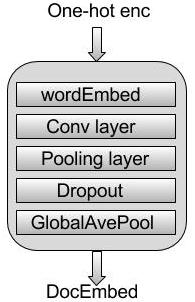
\includegraphics[height=180px]{gfx/4-Design/base_module.png}
		\caption*{Structure of one sequential subnetwork}
		\label{?}
	\end{minipage}\hfill
	\begin{minipage}{0.5\textwidth}
		\centering
		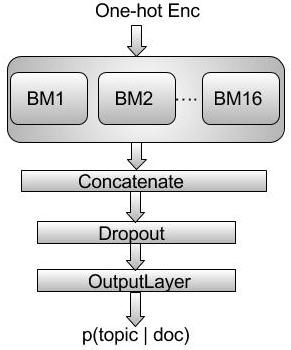
\includegraphics[height=180px]{gfx/4-Design/combined_model.png}
		\caption*{Architecture of the whole combined network}
		\label{?}
	\end{minipage}
\end{figure}

%-----

\section{Early Ticket: MNIST-Lenet-FCN}
As this experiment shares an architecture with the reproduction discussed earlier, redundant subsections are omitted. 
\subsection*{Aim of the Experiment}
In the introduction of this thesis, I remarked that there is no inherent necessity that one defines the structure of lottery tickets after full training of a network. Such a definition is natural, but in the end, J. Frankle and M. Carbin perform network architecture search on the initial network. The trained weights are only used to inform this search.
In principle, searching for a performant architecture could be done without any training, using only the initialized weights, but H. Zhou et al. rule out that possibility in their ablation study.\cite{Deconstructing_LTH} This experiment aims to study the behavior of lottery tickets dependent on the point in training when the weights are used to inform the pruning.
\subsection*{Pruning}
The network converges no later than 15 epochs into training. Thus 15 experiments were performed, each being set to another epoch for pruning. 
To ensure comparability all 15 networks share the same initialization, and each training is run for the full  50 epochs of the original experiment.



\subsection*{Task}
For each document, the network has to determine precisely one out of 30 possible topics.

\subsection*{Architecture and Setup}
% R. Pappagari et al. do not specify the dropout rate. 
Embedding layers are dense layers with one-hot input and special implementation. As such they are pruned like dense layers


%\subsection*{Pruning}
